177. \begin{figure}[ht!]
\center{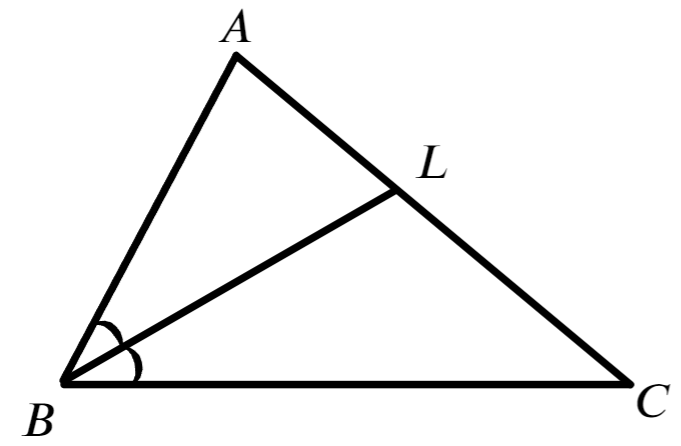
\includegraphics[scale=0.35]{g9-177.png}}
\end{figure}\\
По теореме об основании биссектрисы имеем соотношение $\cfrac{AL}{LC}=\cfrac{AB}{BC}=\cfrac{8}{12}=\cfrac{2}{3}.$ Значит, $AL=\cfrac{2}{5}\cdot AC=\cfrac{2}{5}\cdot10=4.$ Запишем теорему косинусов для треугольника $ABC:\ BC^2=AB^2+AC^2-2\cdot AB\cdot AC\cdot \cos(\angle A),\ 144=64+100-2\cdot8\cdot10\cdot
\cos(\angle A),\ \cos(\angle A)=\cfrac{1}{8}.$ Теперь запишем теорему косинусов для треугольника $ABL:\ BL^2=AB^2+AL^2-2\cdot AB\cdot AL\cdot \cos(\angle A)=
64+16-2\cdot8\cdot4\cdot\cfrac{1}{8}=72,$ откуда $BL=\sqrt{72}=6\sqrt{2}.$\newpage\noindent
